\paragraph{Field} is a force per unit of mass (or, in case of electricity, charge).
\paragraph{Potential} is potential energy per unit of mass (for gravity) or unit of charge (for electricity).
 \subparagraph{Example} Gravitation on Earth's surface is $\vec{F} = -\hat{y}mg$. Then gravitational field is $\vec{g}=-\hat{y}g$ and gravitaional potential is:
 
 $$\phi(\vec{r}) - \phi(\vec{A}) = \int_{\vec{r}}^{\vec{A}} \vec{g} \cdot d\vec{r}$$
 
 \paragraph{Gradient in 2D in polar coordinates}
 
 $$\vec{\nabla} U = \hat{r} \frac{\delta U}{\delta r} + \hat{\theta}\frac{1}{r}\frac{\delta U}{\delta \theta}$$
 
 \paragraph{Potential energy in 1D}
 
 
 \begin{center}
 	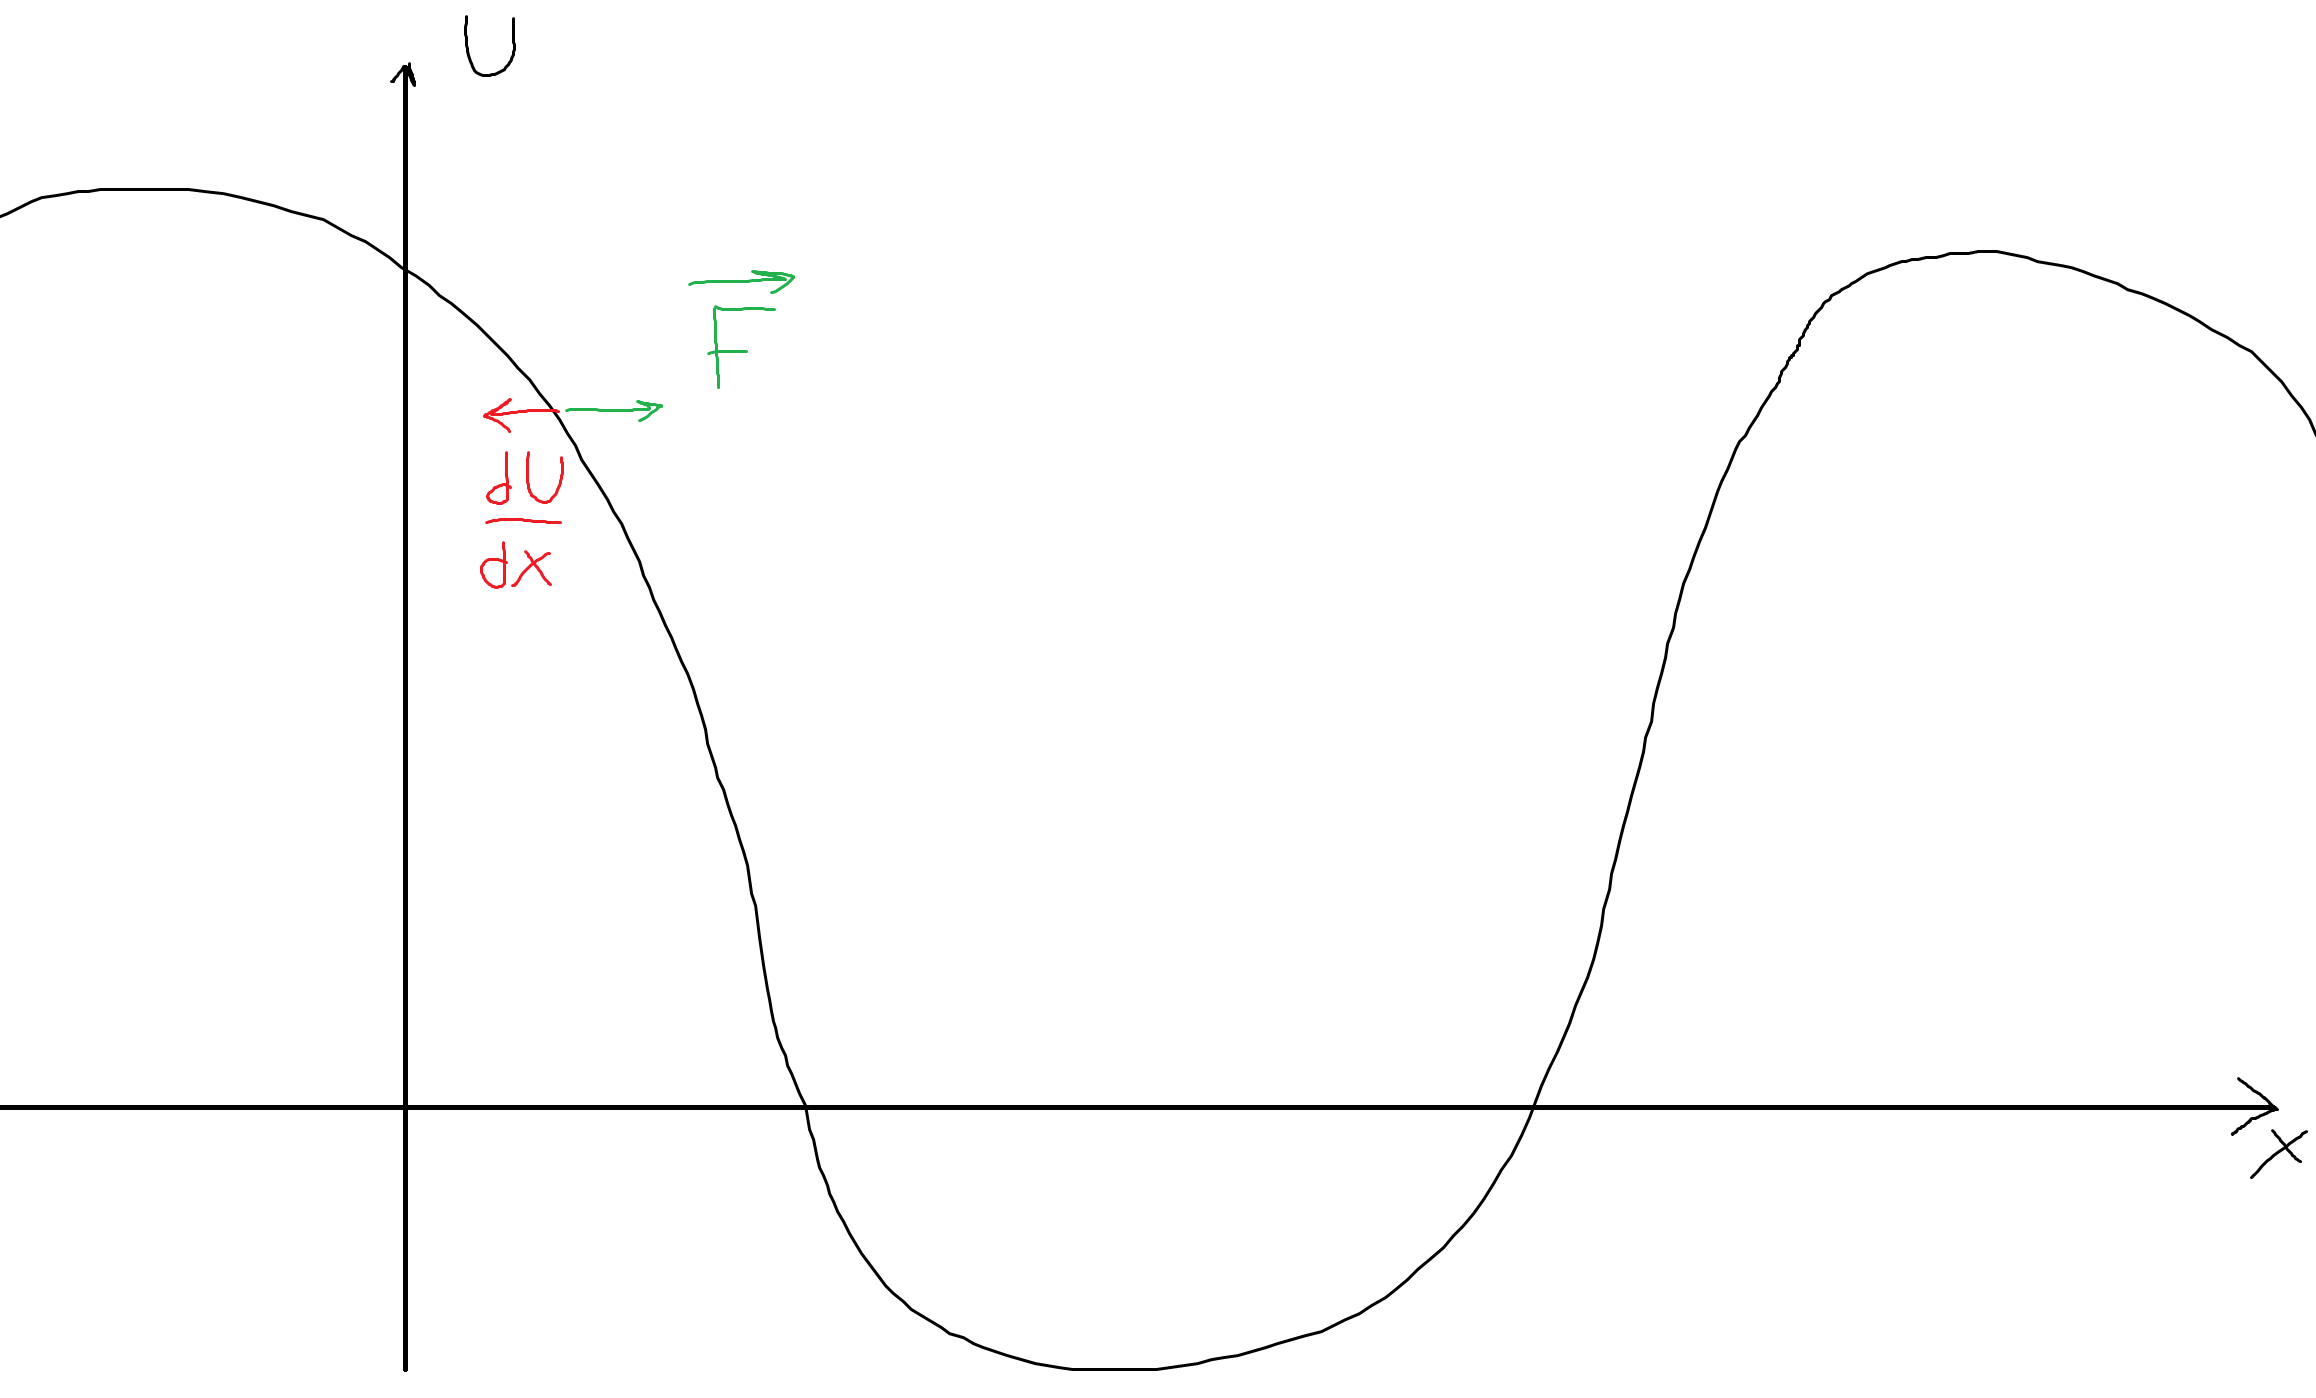
\includegraphics[width=\linewidth]{./lect11/pic1.png}
 	\end{center}
 	
 	\begin{itemize}
 		\item Force acts in direction of low potential
 		\item In points of maximum and minimum of potential force equals to 0.
 		\item \begin{itemize} 
 			\item Maximum point: non-stable equilibrium. $\frac{d^2 U}{dx^2}<0$
 			\item Minimum point: stable equilibrium.$\frac{d^2 U}{dx^2}>0$
 		\end{itemize}
 	\end{itemize}
 	
 	\paragraph{Potential energy between two bodies}
 	
 	

 	\begin{center}
 		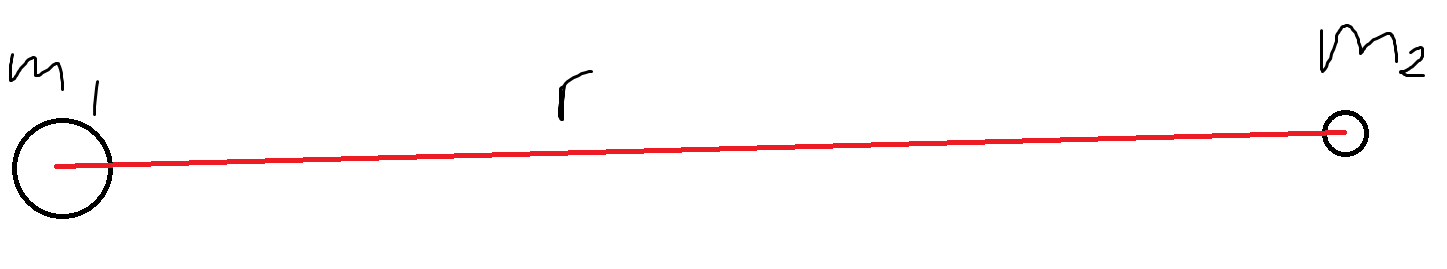
\includegraphics[width=\linewidth]{./lect11/pic2.png}
 	\end{center}
 	$$F = -\hat{r} \frac{Gm_1m_2}{r^2}$$
 	where $m_1, m_2$ - (gravitational) masses and $G$ - gravitational constant.
 	
 	$$U(\vec{r}) - U(\vec{A}) = \int_{\vec{A}}^{\vec{r}} \left( - \vec{F} \right) \cdot d\vec{r} \stackrel{d\vec{r} = \hat{r} dr}{=} \int_{r_A}^{r} \frac{Gm_1m_2}{r^2} dr = \left[ - \frac{G m_1 m_2}{r} \right]^r_{r_A} = -\frac{Gm_1m_2}{r} - \left( - \frac{Gm_1m_2}{r_A}\right)$$
 	
 	We choose reference point $r_A \to \infty$ since $U(\infty) = 0$ and get:
 	
 	$$U(r) = - \frac{G m_1 m_2}{r}$$
 	
 	At Earth's surface:
 	
 	$$U(r) = - \frac{G M_{\bigoplus}}{R_{\bigoplus}}m$$
 	
 	At height h over Earth's surface:
 	
 	$$U(r_h)= - \frac{G M_{\bigoplus}}{R_{\bigoplus}+ h}m = -\frac{G M_{\bigoplus}}{R_{\bigoplus} \left( 1 + \frac{h}{R_{\bigoplus}} \right)}m = - \frac{G M_{\bigoplus}}{R_{\bigoplus}}m + \underbrace{\frac{G M_{\bigoplus}}{R_{\bigoplus}^2}}_{\parbox{1.5cm}{\centering \scriptsize g}}mh$$
 	
 	i.e.
 	
 	$$U(r_h) = U_{floor} + gmh$$
 	
 	
 	\begin{center}
 		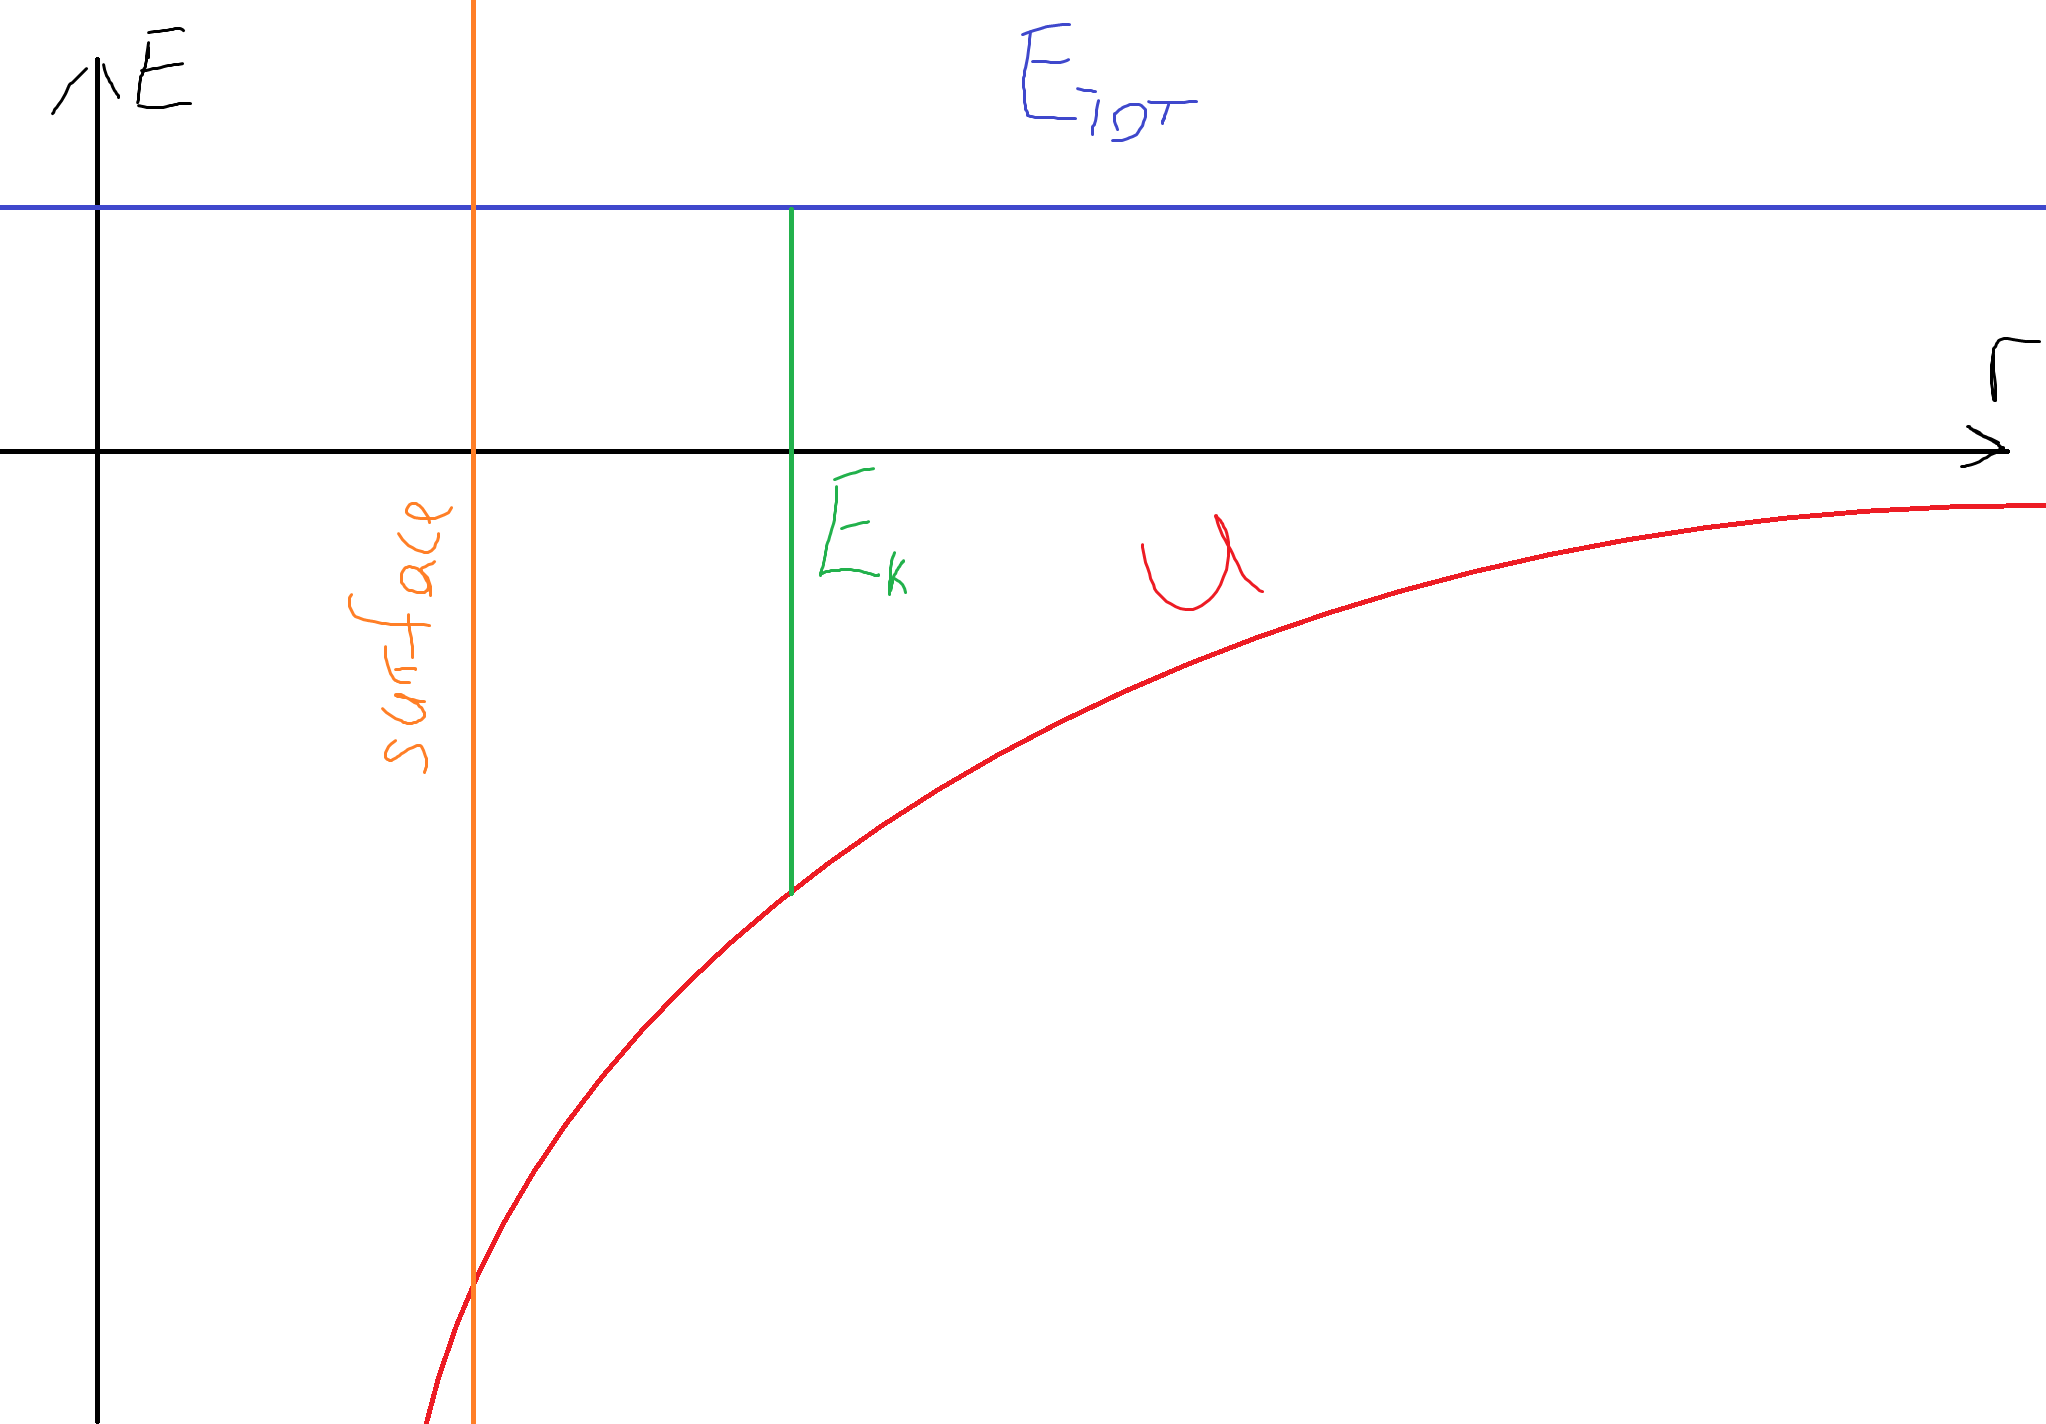
\includegraphics[width=\linewidth]{./lect11/pic3.png}
 	\end{center}
 	
 	\subsection{Conservation of impulse}
 	
 	Let's show that internal forces don't change total impulse. For $N$ bodies:
 	
 	$$\underbrace{\vec{p}}_{\parbox{2cm}{\scriptsize \centering total impulse}} = \sum_{i=1}^{n} \underbrace{m_i \vec{v}_i}_{\parbox{2cm}{\scriptsize \centering impulse of each mass}}$$
 	
 	According to the third law:
 	
 	$$F_{ij} = F_{ji}$$
 	
 	Derive total impulse:
 	
 	$$\frac{d\vec{p}}{dt} =  \sum_{i=1}^{n} \frac{d }{dt} \left( m_i \vec{v}_i \right)$$
 	
 	For two particles:
 	$$\frac{d\vec{p}}{dt} =  \frac{d }{dt} \left( m_1 \vec{v}_1 \right) + \frac{d }{dt} \left( m_1 \vec{v}_1 \right)$$
 	
 	Now substitute  $\frac{d }{dt} \left( m_1 \vec{v}_1 \right) =  \vec{F}_{21}$ and   $\frac{d }{dt} \left( m_2 \vec{v}_2 \right) = \vec{F}_{12}$:
 	
 	$$\frac{d\vec{p}}{dt} = \vec{F}_{12} + \vec{F}_{21} = 0$$
 	
 	\subsection{Mass center}
 	\paragraph{Definition}
 	
 	$$\vec{R}_{cm} = \frac{\sum_{i=1}^{N} \vec{r}_i m_i}{\sum_{i=1}^{N} m_i}$$
 	
 	\paragraph{Example} A second law for a system of masses:
 	
 	$$\vec{F} = \left( \sum_{i=1}^{N} m_i \right) \ddot{\vec{R}}_{cm}$$
